%
% section 7.3.1
%
\subsection{Βασικά Συστατικά Συστήματος Διαχείρισης (MS -- MIB -- AGENT)}

\begin{inthebox}
Ο \emph{Διαχειριστής Δικτύου (Manager Server)} είναι ένας ή περισσότεροι υπολογιστές που διαχειρίζεται τα στοιχεία του δικτύου που έχουν επιλεγεί για αυτό το σκοπό. Ο Manager Server εκτελεί κατάλληλο λογισμικό διαχειριστή το οποίο συχνά εμφανίζει στο διαχειριστή (άνθρωπο) το δίκτυο σε μορφή χάρτη (σχήμα \ref{7-2}) επιτρέποντας του να δει με μια ματιά την κατάσταση όλων των διαχειριζόμενων συσκευών.\\
\end{inthebox}

\begin{figure}[!ht]
 \centering
 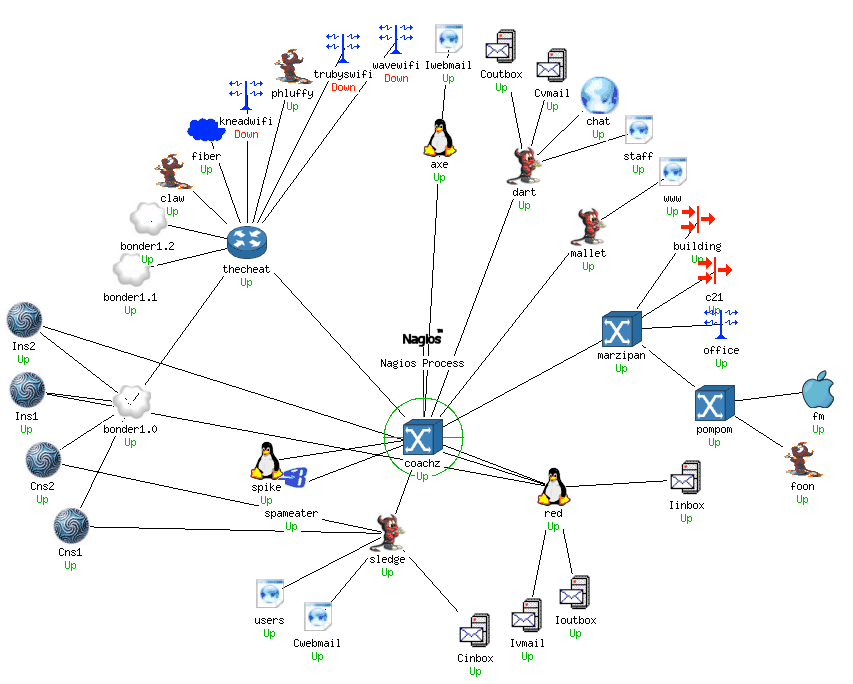
\includegraphics[width=0.95\textwidth]{images/chapter7/7-2}
 \caption {\textsl{Δικτυακός Χάρτης}}
 \label{7-2}
\end{figure}

Το λογισμικό πραγματοποιεί τις παρακάτω λειτουργίες:

\begin{itemize}
\item Αποστέλλει αιτήματα στους αντιπροσώπους που είναι εγκατεστημένοι στο δίκτυο
\item Λαμβάνει απαντήσεις από τους αντιπροσώπους
\item Ορίζει μεταβλητές παρακολούθησης στους αντιπροσώπους. Ουσιαστικά καθορίζει ποια είναι τα μεγέθη που θα μετρώνται. Για παράδειγμα, ο διαχειριστής μπορεί να ορίσει να μετρώνται τα πλαίσια ανα δευτερόλεπτο που διακινούνται σε μια θύρα Ethernet ενός switch. Για το σκοπό αυτό θα στείλει αντίστοιχη οδηγία στον αντιπρόσωπο που εκτελείται στο switch αυτό
\item Παρακολουθεί τους συναγερμούς. Ειδοποιεί τον διαχειριστή (άνθρωπο) όταν οι παράμετροι λειτουργίας του δικτύου είναι εκτός των αποδεκτών ορίων (μπορεί να στείλει ειδοποιήσεις μέσω email, sms κλπ)
\item Προσφέρει κατάλληλο περιβάλλον χρήστη (π.χ. δικτυακό χάρτη) για την καλύτερη παρακολούθηση των πληροφοριών του δικτύου από τον άνθρωπο
\end{itemize}

\begin{inthebox}
Ο \emph{Αντιπρόσωπος Δικτύου} είναι το λογισμικό που εκτελείται σε κάθε δικτυακή συσκευή που είναι υπό διαχείριση.\\
\end{inthebox}

Όπως αναφέραμε και πριν, δεν είναι όλες οι συσκευές δικτύου κατάλληλες για την εκτέλεση λογισμικού αντιπροσώπου. Οι φτηνές συσκευές συνήθως δεν έχουν δυνατότητες διαχείρισης και προσπαθούμε να τις αποφεύγουμε σε δίκτυα μεσαίου / μεγάλου μεγέθους. 

Βασικές λειτουργίες του αντιπροσώπου είναι:

\begin{itemize}
\item Η συλλογή πληροφοριών από τα διαχειριζόμενα αντικείμενα του δικτύου
\item Η διαμόρφωση παραμέτρων των διαχειριζόμενων αντικειμένων. Σε αρκετές διαχειριζόμενες συσκευές είναι δυνατή η αλλαγή ρυθμίσεων με την αποστολή κατάλληλων εντολών από το Manager Server
\item Η απάντηση στα αιτήματα των προγραμμάτων διαχείρισης δικτύου
\item Η δημιουργία και αποστολή συναγερμών στους διαχειριστές
\end{itemize}

\begin{inthebox}
Η \emph{Βάση Πληροφοριών Διαχείρισης ή MIB, Management Information Base} είναι ένα σχήμα αποθήκευσης πληροφοριών σε μορφή βάσης δεδομένων που χρησιμοποιείται για τη διαχείριση των αντικειμένων / οντοτήτων ενός δικτύου. Αντικείμενο θεωρείται εδώ κάθε συσκευή που είναι συνδεδεμένη στο δίκτυο (υπολογιστές, εκτυπωτές, δικτυακές συσκευές, δρομολογητές κλπ).\\
\end{inthebox}

Η δομή της παραπάνω βάσης είναι ιεραρχική και μοιάζει με αντεστραμμένο δέντρο. Κάθε φύλλο είναι ένα διαχειριζόμενο αντικείμενο και αντιστοιχεί σε ένα πόρο του συστήματος. Η εισαγωγή πληροφοριών γίνεται μέσω μιας ακολουθίας αριθμών που προσδιορίζει με μοναδικό τρόπο ένα αντικείμενο (Ταυτοποίηση Αντικειμένου ή Object Identifier).

Οι MIBs συνήθως χρησιμοποιούν δομές πινάκων με πολλές μεταβλητές (πεδία). Οι πίνακες μπορεί να έχουν από μηδέν εγγραφές και άνω και ένα σύστημα διαχείρισης έχει πρόσβαση σε αυτούς για να εκτελέσει τυπικές λειτουργίες βάσεων δεδομένων: εισαγωγή δεδομένων, ανάκτηση (αναζήτηση), ανάκτηση επόμενης / προηγούμενης εγγραφής, ενημέρωση, διαγραφή κλπ.